\documentclass[paper=a4, fontsize=11pt]{article}

\usepackage[english]{babel}
\usepackage{sectsty}
\usepackage{graphicx}
\graphicspath{ {./} }
 

\allsectionsfont{\centering \normalfont\scshape}


\title{\normalfont \normalsize \textsc{KSZ, Kantonsschule Zug} \\ [25pt]
\huge Status Report\linebreak\linebreak \large Maturaarbeit\\ 
}
\author{Nicolà Lohr}


\begin{document}


\maketitle

\newpage
\section{Summary of my status}
So far I created the basic proof of concept like stated in the agreement, more to this later in detail. I learnt the basics for TeX. As proof, I am writing this report in TeX. My books which I had to select are Data Science from Scratch and Data Algorithms. The plan is to read these books during my summer holidays. Both books have Algorithms in them, which I should be able to use in the next phase in my project (Working with different Algorithms and finding there strength and weaknesses). The first book also helps to clean my data and potentially create graphics like I'm going to do. 
For the last point, time-commitment, I will not make a paper/project on the ETH level, I will first focus on doing a great paper on the school level and expand as soon as I have a good result and still have time to go further. 

\section{Proof of Concept}
Now back to my code. So far I programmed a basic proof of concept which finds out in which class a person (student or teacher) is, only given the mac-address of the person. It uses the data provided by the IT-department of the school and the time-table which is available online, but to make it easier I got a parsed version (similar to XML) so I hadn't to do this on my own. 
The first step of my code is to read in all the data and parse it correctly. I transformed the timetable XML into a dictionary. The dictionary has three levels. The first level is the day (0-6), the second one is the lesson start (e.g "0740") and the third is the room (e.g. "P03") and there the class and teacher, which have school then, are stored there. So to find out which class is in the room 347 at a Thursday from 10:30, you can call the dictionary (d) like this: d[3]["1030"]["347"] and the result would be ["5H", "KELL"]. 

To parse the logfiles I just looked at it and retrieved the information I need (user mac, access-point mac and time). Then I got a list with all datapoints encoded as tuples. The list also gets filtered to just use the user-macs of the person of interest.

To find which class the person is in, I compare every data point from the list with the time table. For that, I first check in which lesson this data point was taken, or at least before which one. Then it is a simple dictionary look up to find the teacher and the class which I save in another list. Then I just have to count how many times a class or teacher are on the list and find the one who has the most "hits". The runtime is okay with about one minute for having over half a year of data. (How exact it is I haven't done yet?) 

I also did a reverse lookup, this means I didn't apply the filter for the data and look at all macs of the students and teachers. It has about the same processing time because the analysis of the data part is just a small fast part of the program.

\section{Friends-Tracking}
As a side-project I did, which is not on the to-do list, but I think it is noticeable, I tried to find friends of somebody with the log-files. I looked for how many people walked together so that their phone switches the access-point at about the same time (~5 sec). I mostly found people who are in the same class together but also had some successes with other students.

\section{Paper}
I started with the paper, I wrote the table of contents and I am going to start soon with the content, especially the result I already got and the one I don't have to code.

\newpage
\section{Brainstorm}
Here is the brainstorming from one of the meetings with Wiwi:


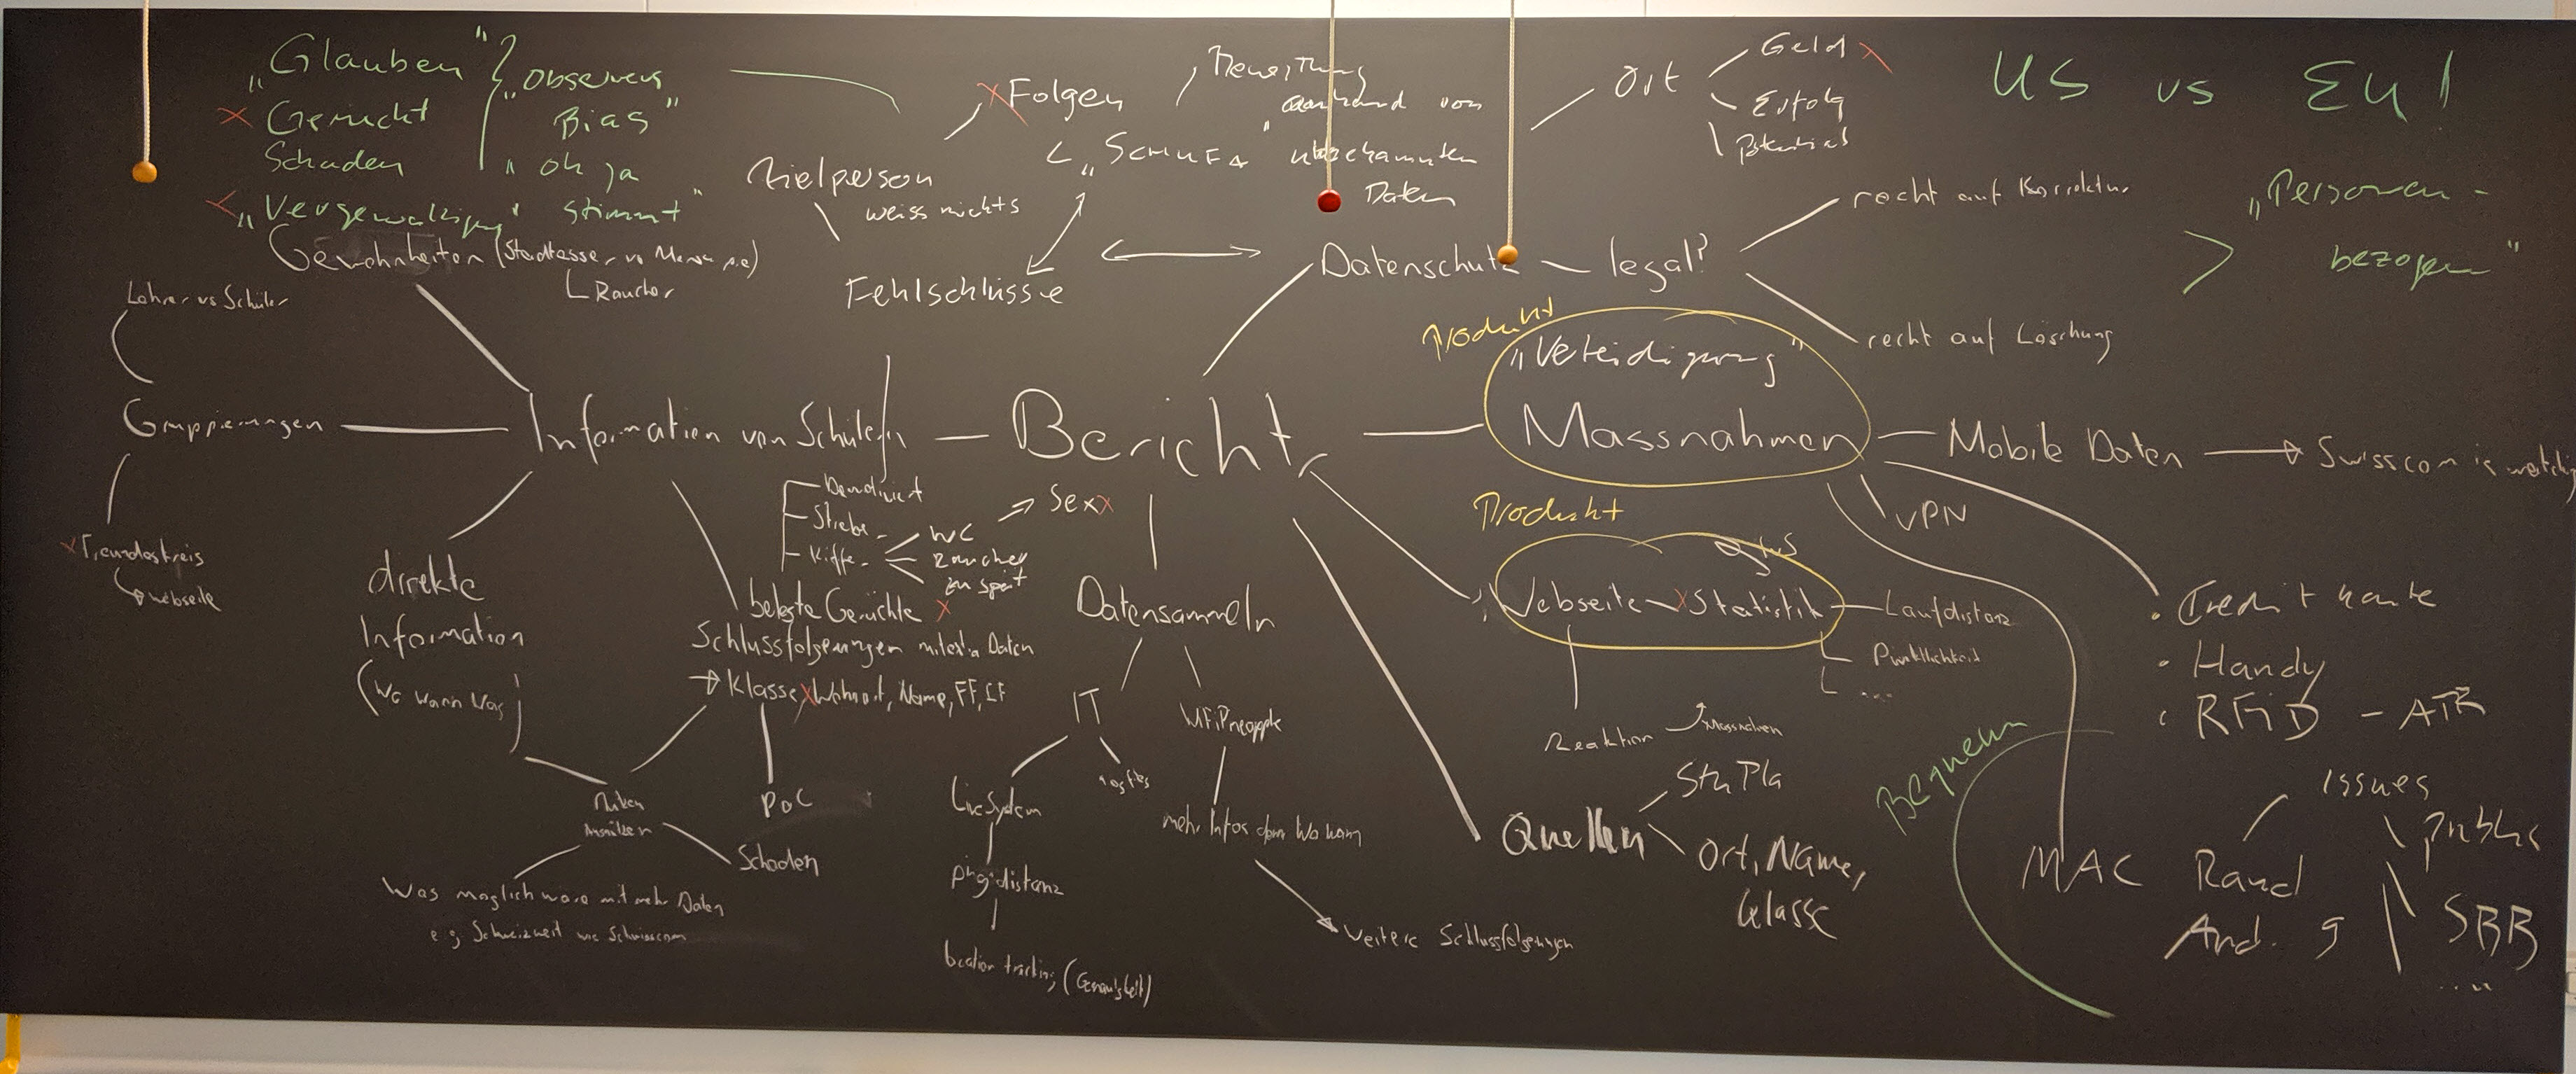
\includegraphics[width=\textwidth]{brainstorming}

It shows about what I am going to discuss in my paper. What topic I am going to invest time in and where my focus is.
\end{document}